\documentclass[10pt, twocolumn]{article}

\usepackage[a4paper, margin=2cm]{geometry}
\usepackage{amsmath, amssymb}
\usepackage{graphicx}
\usepackage{float}
\usepackage[ruled,vlined]{algorithm2e}
\SetKwFor{KwParallel}{parallel}{do}{end}
\SetKw{KwLaunch}{launch}

\usepackage{tikz}
\usetikzlibrary{arrows.meta, positioning}

\title{
    
\includegraphics[width=2cm]{logo.png}\\[0.3cm]
    \textbf{Mining Proportional Patterns in Online Retail Data}
}

\author{
    Matteo Baldi \\
    \textit{VR536965}
    \and
    Mattia Cappelletti \\
    \textit{VR543935}
}

\date{}

\begin{document}

\maketitle

% ============================================================
\section{Introduction}
% ============================================================

Frequent Itemset Mining (FIM) has long been a cornerstone of market basket
analysis, providing retailers with the ability to discover hidden associations
between products purchased together.
The evolution of these techniques led to the development of the FP-Growth
algorithm, which revolutionised the field by adopting a divide-and-conquer
approach that avoids the prohibitively expensive candidate generation typical
of earlier methods like Apriori.
However, in the era of massive online retail datasets, two primary challenges
emerge: computational scalability and the inherent limitation of binary data.

\subsection{The Challenge of Scale and the Long Tail}

Modern retail databases often reach sizes where memory and computational costs
on a single machine become unsustainable.
Furthermore, web-based retail data frequently exhibits a ``long-tail''
distribution, where a massive number of items have low individual support but
represent a significant portion of overall revenue when considered collectively.
To address this, the Parallel FP-Growth (PFP) framework was introduced,
enabling the distribution of mining tasks across a cluster of machines using a
five-step MapReduce-based pipeline.
PFP achieves virtually linear speedup by sharding the transaction database into
independent tasks, eliminating the need for inter-machine communication during
the mining process.

\subsection{Moving Beyond Binary Mining}

Despite the efficiency of PFP, traditional FIM frameworks are largely limited
to the binary presence or absence of items, effectively ignoring the purchased
quantities.
In a retail context, understanding the exact proportions of items bought
together (e.g., a ``2-for-4'' ratio of related products) provides deeper
insights for bundle recommendations, targeted upselling, and inventory
management.

\subsection{The Proposed Extension: Proportional Analysis}

This project proposes a structural extension to the PFP framework designed to
extract proportional quantitative relationships. By implementing a custom
Bijective Token Indexing phase, we adapt the PFP distributed engine to handle
quantitative tuples without modifying its core prefix-tree logic.
The primary contribution of this work lies in the post-mining analytical layer:
we apply a Greatest Common Divisor (GCD) decomposition to identify the
Canonical Shape of frequent patterns — the irreducible proportional ratio of
items.
This logic allows us to bridge the gap between tree-based mining and structural
graph analysis, culminating in a Proportional Relationship Graph.
By applying transitive reduction to these results, we eliminate redundant
informational pathways, providing an optimised, hierarchical atlas of consumer
purchase trajectories that highlights the structural evolution of consumer
behaviour.

% ============================================================
\section{Formal Methodology: Quantitative Itemsets, Canonical Shapes,
  and Scaling Factors}
% ============================================================

To rigorously analyse co-occurrences in retail data while accounting for
purchased quantities, we establish a formal mathematical framework [1, 2]. Let
$I = \{i_1, i_2, \dots, i_m\}$ be the universe of distinct items [3]. A
\textbf{quantitative itemset} $X$ is defined as a set of ordered pairs
representing items and their specific purchased quantities:
$X = \{ (i_j, q_j) \mid i_j \in I,\, q_j \in \mathbb{Z}^+ \}$ [3].

For any frequent quantitative pattern $P \in \mathcal{P}$ characterised by
the quantity set $\{q_1, q_2, \dots, q_k\}$, we define the \textbf{Scaling
Factor} $\alpha$ as the greatest common divisor of those quantities:
$\alpha = \gcd(q_1, q_2, \dots, q_k)$ [4]. This extraction of a common scalar
is theoretically grounded in the \textbf{Prefix Path Property}, which states
that for any node $a_i$ in a path $P$ within an FP-tree, the frequency count
of every node in its prefix subpath must carry the same count as node $a_i$
[5]. In a quantitative context, this property suggests that items appearing in
a single path often co-occur in fixed ratios, justifying the use of a scaling
factor to represent the magnitude of the transaction [4, 5].

Consequently, each pattern $P$ can be uniquely decomposed into its
\textbf{Canonical Shape} $S$, which represents the irreducible proportional
ratio of the items [4]. The shape $S$ is derived by normalising each quantity
in the pattern by the scaling factor:
\begin{equation}
    S = \left\{ \left(i_j, \frac{q_j}{\alpha}\right) \mid (i_j, q_j) \in P
    \right\}
\end{equation}
By sorting these items in a fixed lexicographical order, we ensure a unique
representation for each structural relationship [4, 6, 7]. Under this
formulation, any extracted frequent pattern is represented as a scalar multiple
of its base structure: $P = \alpha \cdot S$ [4].

% ============================================================
\section{Distributed Architecture}
% ============================================================

The massive scale of modern retail transactions necessitates a distributed
computing approach to avoid memory overflows and prohibitive computational
costs [3, 4]. Our architecture leverages the \textbf{Parallel FP-Growth (PFP)}
framework [5], adapted to process quantitative itemsets through a multi-stage
MapReduce-based pipeline. This architecture ensures virtually linear speedup by
eliminating inter-node communication during the mining process [3, 6].

\subsection{Bijective Token Indexing and Vocabulary Discovery}

Standard FIM algorithms are designed to process discrete tokens rather than
complex tuples. To bridge this gap without modifying the underlying
prefix-tree logic, we implement a \textbf{Bijective Token Indexing} phase
(adapted from PFP's Parallel Counting step [7, 8]).
\begin{itemize}
    \item \textbf{Sharding:} The raw transactional database $DB$ is
          partitioned into $P$ independent shards across the cluster [1].
    \item \textbf{Parallel Counting:} Each mapper discovers the local
          vocabulary of $(item, quantity)$ pairs. The MapReduce infrastructure
          aggregates these counts to generate a global \textbf{F-List} [7, 9].
    \item \textbf{Tokenisation:} Every unique pair is mapped to a synthetic
          integer identifier $ID \in \mathbb{Z}^+$. This standardises the input
          for the PFP engine, ensuring that a purchase of ``2 colas'' is treated
          as a distinct frequent entity from ``1 cola'' [10].
\end{itemize}

\subsection{Workload Partitioning and the Group List}

A critical challenge in distributed FP-Growth is balancing the computational
load. PFP addresses this by dividing the $|I|$ items from the F-List into $Q$
independent groups, creating a \textbf{Group List (G-list)} [7].
Each group is assigned a unique \textit{group-id (gid)}. By setting $Q$
significantly higher than the number of physical machines ($P$), we ensure
that if one node finishes its mining task early, it can immediately process
the next group, preventing straggler nodes from bottlenecking the
pipeline [11, 12].

\subsection{Independent Parallel Mining}

The core of the architecture lies in the \textbf{Parallel FP-Growth
Step} [13]. This stage transforms the database into group-dependent
transactions:
\begin{enumerate}
    \item \textbf{Mapper Phase:} Each mapper reads the G-list and outputs
          group-dependent transactions. For each item in a transaction, it emits
          a key-value pair where the key is the \textit{gid} and the value is
          the prefix path of that item [13, 14].
    \item \textbf{Reducer Phase:} Reducers receive independent shards of
          group-dependent transactions. Each reducer builds a \textbf{local
          FP-tree} and mines it recursively to extract patterns [15, 16].
\end{enumerate}
Because the shards are mathematically independent, there is no need for
synchronisation between workers during the recursive tree-growth process,
which is the primary reason for PFP's high scalability [3, 5].

\subsection{Max-Heap Aggregation}

To manage the potentially combinatorial number of patterns, each reducer
maintains a \textbf{Max-Heap ($HP$)} of size $K$ [17, 18]. Instead of
emitting all discovered patterns, the reducer retains only the top-$K$ most
supported patterns per item. This filtered output is aggregated in the final
step to produce the global top-$K$ result, which serves as input for the
Proportional Graph Construction phase.

% ============================================================
\section{Implementation \& Algorithm Design}
% ============================================================

The proposed computational pipeline is engineered to bridge the gap between
distributed statistical mining and structural relationship modelling. The
implementation is divided into three functional phases, each addressing a
specific challenge of quantitative big data processing within an Apache Spark
environment.

\subsection{Phase 1: Distributed Dataset Transformation}

Standard Frequent Itemset Mining (FIM) engines, including the PFP framework,
are designed to process discrete, non-quantitative tokens. To preserve
purchased quantities without altering the underlying prefix-tree logic, we
implement a \textit{Bijective Token Indexing} phase.

This phase executes a distributed transformation where every unique
$(\text{item}, \text{quantity})$ tuple discovered across the database is
assigned a continuous synthetic identifier $ID \in \mathbb{Z}^{+}$. By
leveraging Spark's \texttt{zipWithIndex} operation, we effectively perform the
vocabulary discovery described in Step 2 of the PFP framework. This
pre-processing ensures that quantitative variations (e.g., \texttt{cola:1}
vs.\ \texttt{cola:2}) are treated as distinct frequent entities, maintaining
the granularity required for proportional analysis.

\begin{algorithm}[H]
    \caption{Bijective Token Indexing}
    \KwIn{Transaction database $DB$ with $(item, quantity)$ tuples}
    \KwOut{Transformed database $DB'$ with integer IDs}

    \KwParallel{for each transaction $T \in DB$}{
        extract all pairs $(i, q)$\;
    }
    aggregate global vocabulary of unique $(i, q)$ pairs\;
    assign unique $ID \in \mathbb{Z}^+$ using \texttt{zipWithIndex}\;
    \KwParallel{for each transaction $T \in DB$}{
        replace each $(i, q)$ with corresponding $ID$\;
    }
    \Return{$DB'$}\;
\end{algorithm}

\subsection{Local FP-Growth Mining}

The local FP-Growth procedure was implemented from scratch rather than
delegating to MLlib's built-in \texttt{FPGrowth}, which operates on discrete
tokens and cannot handle the quantitative tuples produced by the Bijective
Token Indexing phase. The implementation centres on a custom \texttt{FPTree}
class that maintains an explicit header table — a dictionary mapping each item
to the list of its nodes in the tree — enabling direct traversal during
conditional tree construction without a full tree scan.

A correctness-critical design choice lies in the conditional pattern base
construction: every prefix node is assigned the count of the conditioning item
rather than its own count. This ensures that the support of any pattern
discovered in the conditional tree is bounded by the frequency of the
conditioning item, as required by the Prefix Path Property. Deviating from
this — for instance, preserving original node counts — would inflate support
estimates and produce spurious frequent patterns.

When a conditional tree reduces to a single path, all nodes inherit the same
count from the conditioning item, making support-based ranking among
combinations redundant. Our implementation exploits this by enumerating
combinations in strictly ascending order of cardinality, retaining only the
first $K$. Beyond correctness, this ordering is a deliberate system-level
trade-off: shorter patterns incur lower serialisation overhead during the
\texttt{combineByKey} shuffle, reducing inter-node communication cost. This is
particularly relevant in long-tail datasets where a disproportionate number of
conditional trees reduce to single paths.
Our implementation adopts a \textit{binary enumeration} scheme over the
path nodes. Nodes are indexed $0, 1, \dots, n{-}1$ from root to leaf.
Each integer mask $m \in \{1, \dots, 2^n - 1\}$ defines a unique
non-empty subset: bit $i$ of $m$ set indicates that node $P[i]$ is
included in the combination. Iterating masks in ascending integer order
from 1 to $2^n - 1$ thus provides a deterministic, canonical enumeration
of all $2^n - 1$ non-empty subsets, stopped after $K$ combinations. This
scheme produces a reproducible, path-length-independent ordering that is
well-suited to bit-manipulation optimisations, with a hard upper bound of
$\min(K,\ 2^n - 1)$ subsets regardless of path length, preserving the
memory guarantee of the heap.

\begin{algorithm}[H]
    \caption{\textsc{TopKCombinations} — binary enumeration}
    \KwIn{Single-path nodes $\mathcal{P} = [p_0, \dots, p_{n-1}]$
          (root to leaf), budget $K$}
    \KwOut{$K$ sub-patterns of $\mathcal{P}$ }

    $count \leftarrow 0$\;
    \For{$mask \leftarrow 1$ \KwTo $2^{|\mathcal{P}|} - 1$}{
        \lIf{$count \geq K$}{\Return}
        $C \leftarrow \bigl(p_i \mid \text{bit } i \text{ of } mask
            \text{ is set},\ i = 0,\dots,|\mathcal{P}|{-}1\bigr)$\;
        yield $C$\;
        $count \leftarrow count + 1$\;
    }
\end{algorithm}
% \begin{algorithm}[H]
%     \caption{\textsc{TopKCombinations} — cardinality-ascending enumeration}
%     \KwIn{Single-path nodes $\mathcal{P}$, budget $K$}
%     \KwOut{First $K$ combinations in ascending cardinality order}

%     $count \leftarrow 0$\;
%     \For{$r \leftarrow 1$ \KwTo $|\mathcal{P}|$}{
%         \For{each combination $C$ of size $r$ from $\mathcal{P}$}{
%             \lIf{$count \geq K$}{\Return}
%             yield $C$\;
%             $count \leftarrow count + 1$\;
%         }
%     }
% \end{algorithm}

Pattern volume is controlled through a Max-Heap of size $K$, maintained
locally by each worker. When the heap exceeds capacity, the lowest-support
pattern is evicted. Local heaps are merged in the aggregation phase via
\texttt{combineByKey}, which ensures the merging is associative and commutative
— a requirement for correct distributed reduction. The choice of $K$ directly
governs the precision-scalability trade-off: a larger $K$ retains more
structural information but increases shuffle volume and memory pressure on the
aggregator nodes.

\begin{algorithm}[H]
    \caption{Local Top-$K$ FP-Growth}
    \KwIn{FP-tree $T$, minimum support $\xi$, suffix $\sigma$, heap size $K$}
    \KwOut{Top-$K$ frequent patterns with support}

    \If{$T$ reduces to a single path $\mathcal{P}$}{
        $H \leftarrow [\,]$\;
        \For{each $C \in \textsc{TopKCombinations}(\mathcal{P},\, K)$}{
            $sup \leftarrow C[0].count$\;
            \If{$sup \geq \xi$}{
                append $\bigl(sup,\ \mathrm{items}(C) + \sigma\bigr)$ to $H$\;
            }
        }
        \Return{$H$}\;
    }
    $\mathcal{H} \leftarrow [\,]$\;
    \For{each $(item,\, nodes)$ in header table of $T$}{
        $sup \leftarrow \displaystyle\sum_{n \,\in\, nodes} n.count$\;
        \lIf{$sup < \xi$}{\textbf{skip}}
        $\pi \leftarrow (item,) + \sigma$\;
        $\mathcal{H} \leftarrow
            \textsc{AddToHeap}(\mathcal{H},\,(sup,\,\pi),\,K)$\;
        $T' \leftarrow \textsc{ConditionalTree}(T,\, item,\, \xi)$\;
        \If{$T'$ is non-empty}{
            $\mathcal{H}' \leftarrow
                \textsc{TopKFPGrowth}(T',\,\xi,\,\pi,\,K)$\;
            $\mathcal{H} \leftarrow
                \textsc{MergeHeaps}(\mathcal{H},\,\mathcal{H}',\,K)$\;
        }
    }
    \Return{$\mathcal{H}$}\;
\end{algorithm}

\subsection{Phase 2: Parallel Pattern Extraction}

With the database standardised into ID sequences, the system triggers the
Parallel FP-Growth engine. The transaction database is divided into independent
shards, allowing each worker to execute local mining tasks without
inter-machine communication. Each shard is processed by a dedicated reducer
that builds a local FP-tree and invokes Algorithm 3 recursively. Once mining
is complete, an inverse mapping $M^{-1}$ is applied to restore the structural
$(item, quantity)$ tuples for final analysis.

\begin{algorithm}[H]
    \caption{Parallel FP-Growth with Top-$K$ Filtering}
    \KwIn{Transformed database $DB'$, parameter $K$}
    \KwOut{Top-$K$ frequent patterns}

    partition $DB'$ into independent shards\;
    \KwParallel{for each shard}{
        build local FP-tree\;
        \For{each discovered pattern $P$ via Algorithm 3}{
            insert into Max-Heap $HP$ of size $K$ based on support\;
            prune if $|HP| > K$\;
        }
    }
    aggregate all local heaps\;
    apply inverse mapping $M^{-1}$ to recover $(item, quantity)$ tuples\;
    \Return{Top-$K$ patterns}\;
\end{algorithm}

\subsection{Phase 3: Proportional Graph Construction}

The final phase transforms the flat list of frequent quantitative patterns
into a hierarchical Directed Acyclic Graph (DAG) by exploiting the
mathematical structure of their scaling factors.

\subsubsection{GCD Decomposition}

For each extracted pattern, the system computes the Scaling Factor $\alpha$
and the Canonical Shape $S$ via a parallel GCD calculation. Patterns are then
clustered by identical shape using Spark's \texttt{groupByKey}, which routes
all patterns sharing the same structural ratio to a single worker node —
ensuring that the subsequent graph construction is both locally complete and
globally independent across shape groups.

\subsubsection{Transitive Modulo Pruning}

Within each shape group, the algorithm performs a pairwise divisibility check
over the set of scaling factors $V = \{\alpha_1, \dots, \alpha_n\}$. An edge
$(\alpha_i, \alpha_j)$ is created if $\alpha_j \bmod \alpha_i = 0$,
signifying a perfect scalar transition. Raw edge generation is then refined
by transitive reduction: any direct edge $(P_i, P_j)$ is pruned if an
intermediate node $P_k$ exists such that $P_i \rightarrow P_k \rightarrow
P_j$. This eliminates informational redundancy while preserving all
structurally meaningful scaling increments. The local
$\mathcal{O}(|\alpha|^2)$ cost of this check is acceptable because each
group is processed independently, keeping the global phase parallelisable
across shape groups.

\begin{algorithm}[H]
    \caption{Proportional Graph Construction with Transitive Modulo Pruning}
    \KwIn{Set of frequent patterns $\mathcal{P}$}
    \KwOut{Directed Acyclic Graph (DAG)}

    \KwParallel{for each pattern $P \in \mathcal{P}$}{
        compute $\alpha = \gcd(q_1, \dots, q_k)$\;
        compute canonical shape $S = P / \alpha$\;
    }
    group patterns by identical $S$ using \texttt{groupByKey}\;
    \KwParallel{for each group $S$}{
        let $V = \{\alpha_1, \dots, \alpha_n\}$\;
        \ForEach{$(\alpha_i, \alpha_j)$ with $\alpha_i < \alpha_j$}{
            \If{$\alpha_j \bmod \alpha_i = 0$}{
                create edge $(P_i, P_j)$\;
            }
        }
        remove $(P_i, P_j)$ if $\exists\, P_k$ such that
        $P_i \rightarrow P_k \rightarrow P_j$\;
    }
    \Return{DAG}\;
\end{algorithm}

To clarify the procedure of Section~4.4, we present a minimal synthetic
example covering both the linear scaling topology and the multi-parent
convergence case.

The example considers two disconnected frequent structures: a three-item
Beverage association with base ratio $1{:}2{:}3$ (cola, juice, water) and a
two-item Pancake association with base ratio $2{:}1$ (flour, milk).
Table~\ref{tab:gcd_decomposition} summarises the GCD decomposition of the
patterns extracted by the PFP engine. Despite varying absolute quantities,
each group maps to a single canonical shape, confirming that the tokenisation
and inverse mapping steps preserve proportional structure correctly.

\begin{table*}[h]
    \centering
    \begin{tabular}{|c|c|c|c|c|}
        \hline
        \textbf{Group} & \textbf{Pattern} & $\mathbf{\gcd(\cdot)}$ &
        \textbf{Canonical Shape ($S$)}                              &
        \textbf{Scale ($\alpha$)}                                                                                            \\
        \hline
        $G_{S_1}$      & $P_1$            & $\gcd(1,2,3)=1$        &
        $\{(\text{cola},1),(\text{juice},2),(\text{water},3)\}$     & 1                                                       \\
                       & $P_2$            & $\gcd(2,4,6)=2$        &
        $\{(\text{cola},1),(\text{juice},2),(\text{water},3)\}$     & 2                                                       \\
                       & $P_3$            & $\gcd(3,6,9)=3$        &
        $\{(\text{cola},1),(\text{juice},2),(\text{water},3)\}$     & 3                                                       \\
                       & $P_4$            & $\gcd(6,12,18)=6$      &
        $\{(\text{cola},1),(\text{juice},2),(\text{water},3)\}$     & 6                                                       \\
        \hline
        $G_{S_2}$      & $P_5$            & $\gcd(2,1)=1$          &
        $\{(\text{flour},2),(\text{milk},1)\}$                      & 1                                                       \\
                       & $P_6$            & $\gcd(4,2)=2$          &
        $\{(\text{flour},2),(\text{milk},1)\}$                      & 2                                                       \\
                       & $P_7$            & $\gcd(8,4)=4$          &
        $\{(\text{flour},2),(\text{milk},1)\}$                      & 4                                                       \\
        \hline
    \end{tabular}
    \caption{GCD decomposition into canonical shapes and scaling factors
        for the two synthetic consumer behaviours.}
    \label{tab:gcd_decomposition}
\end{table*}

The Beverage group $G_{S_1}$ exercises the multi-parent convergence case.
The scale set $V_{S_1} = \{1,2,3,6\}$ admits three raw divisibility edges
from $P_1$: toward $P_2$, $P_3$, and $P_4$. The transitive reduction
correctly identifies that $P_4$ is reachable from $P_1$ via both
$1 \rightarrow 2 \rightarrow 6$ and $1 \rightarrow 3 \rightarrow 6$, and
prunes the redundant direct edge $(P_1, P_4)$ while preserving $(P_2, P_4)$
and $(P_3, P_4)$ — since $2 \nmid 3$ and $3 \nmid 2$, these represent
genuinely independent scaling paths. The Pancake group $G_{S_2}$ exercises
the simpler linear case: $V_{S_2} = \{1,2,4\}$ yields a clean chain
$P_5 \rightarrow P_6 \rightarrow P_7$ with no redundant edges. Both
resulting DAGs are shown in Figure~\ref{fig:dags}.

\begin{figure*}[h]
    \centering
    \begin{minipage}{0.48\textwidth}
        \centering
        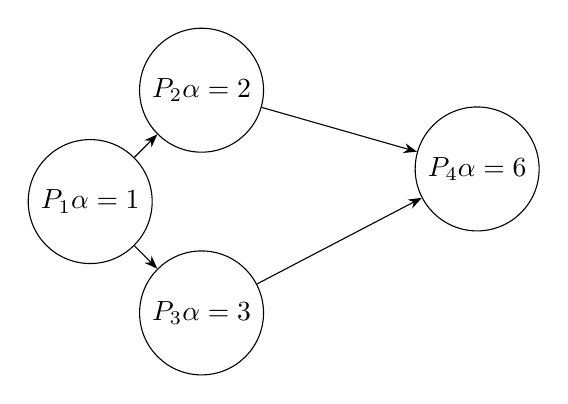
\begin{tikzpicture}[
                node distance=2cm,
                every node/.style={circle, draw, minimum size=1cm},
                >=Stealth
            ]
            \node (P1) {$P_1$\\$\alpha=1$};
            \node (P2) [above right of=P1] {$P_2$\\$\alpha=2$};
            \node (P3) [below right of=P1] {$P_3$\\$\alpha=3$};
            \node (P4) [right of=P2, xshift=1.5cm, yshift=-1cm]
                {$P_4$\\$\alpha=6$};
            \draw[->] (P1) -- (P2);
            \draw[->] (P1) -- (P3);
            \draw[->] (P2) -- (P4);
            \draw[->] (P3) -- (P4);
        \end{tikzpicture}
        \vspace{0.2cm}
        \textbf{(a) Beverage $G_{S_1}$: multi-parent convergence}
    \end{minipage}
    \hfill
    \begin{minipage}{0.48\textwidth}
        \centering
        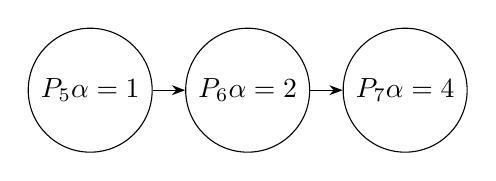
\begin{tikzpicture}[
                node distance=2cm,
                every node/.style={circle, draw, minimum size=1cm},
                >=Stealth
            ]
            \node (P5) {$P_5$\\$\alpha=1$};
            \node (P6) [right of=P5] {$P_6$\\$\alpha=2$};
            \node (P7) [right of=P6] {$P_7$\\$\alpha=4$};
            \draw[->] (P5) -- (P6);
            \draw[->] (P6) -- (P7);
        \end{tikzpicture}
        \vspace{0.2cm}
        \textbf{(b) Pancake $G_{S_2}$: linear scaling chain}
    \end{minipage}
    \caption{DAGs produced by the transitive reduction step on the synthetic
        example. (a) exercises multi-parent convergence; (b) exercises linear
        scaling. In both cases the algorithm produces the minimal edge set.}
    \label{fig:dags}
\end{figure*}
\newpage
% ============================================================
\section{Experimental Evaluation}
\begin{figure*}[t]
    \centering
    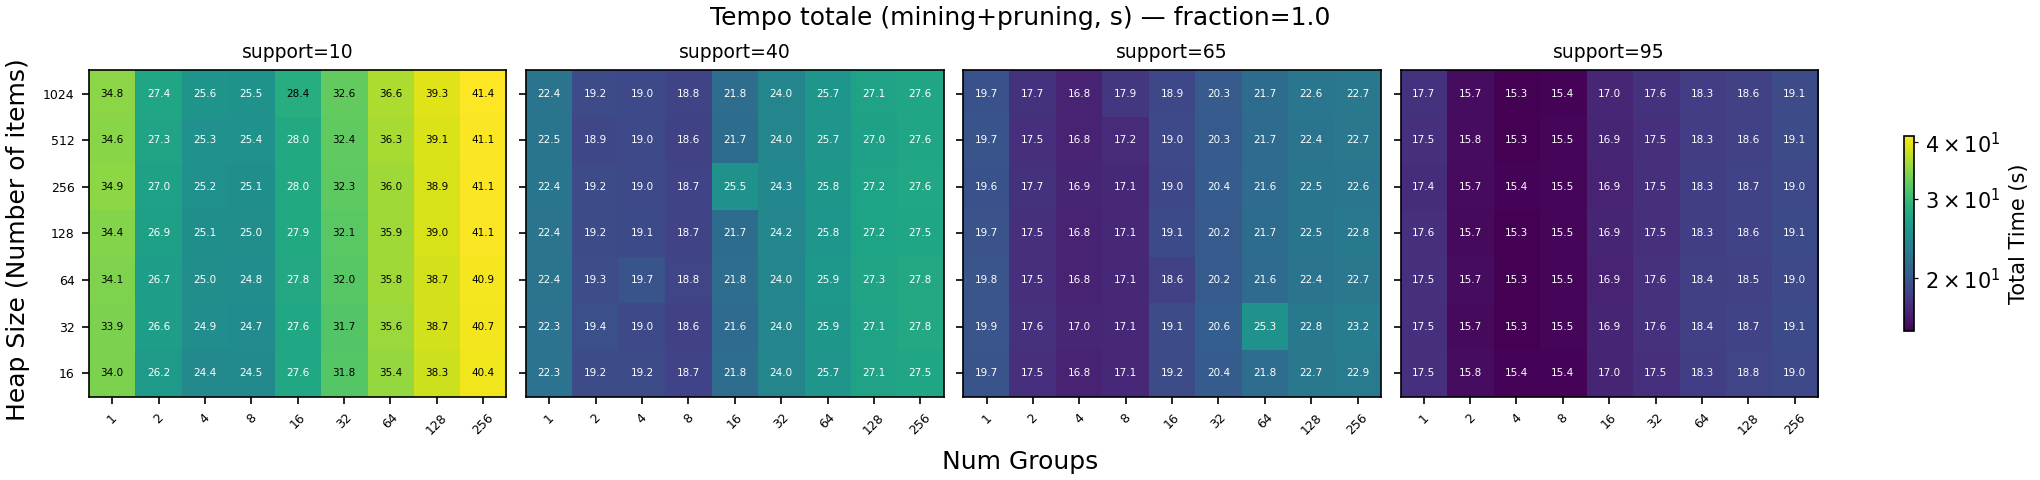
\includegraphics[width=\textwidth]{7_heatmap_groups_heap.png}
    \caption{Total execution time (mining + pruning) as a function of
        heap size $K$ (y-axis) and number of groups $Q$ (x-axis), at
        four support levels on the full dataset ($f{=}1.0$). Heap size
        has no measurable effect on execution time, consistent with the
        absence of network overhead in \texttt{local[*]} mode. The
        number of groups shows modest sensitivity at low support, where
        task scheduling overhead becomes relevant.}
    \label{fig:heatmap}
\end{figure*}
This section evaluates the computational performance and output
characteristics of the proposed pipeline on the Dunnhumby \textit{The
Complete Journey} dataset. All experiments were executed locally using
Apache Spark in \texttt{local[*]} mode, leveraging all available cores.

\subsection{Dataset and Experimental Setup}

The Dunnhumby dataset contains $2{,}595{,}732$ purchase records from
2,500 households over 52 weeks, covering approximately $92{,}000$ unique
products. After grouping records by basket identifier, the dataset yields
approximately $280{,}000$ unique transactions. The quantity distribution
is highly skewed: while the median purchase quantity is 1 unit, the mean
is approximately 100 and the maximum reaches $89{,}638$ units, reflecting
the extreme long-tail characteristic of real-world retail data. This skew
directly stresses the GCD-based canonical shape extraction, as outlier
quantities can suppress the discovery of proportional relationships —
a limitation discussed in Section~\ref{sec:limitations}. Negative
quantities representing product returns are handled transparently by the
absolute-value normalisation applied during tokenisation.

Experiments were conducted as a partial grid search over the following
ranges: minimum support $\xi \in \{10, 15, \dots, 100\}$, heap size
$K \in \{16, 32, \dots, 1024\}$, number of groups $Q \in \{1, 2, 4,
\dots, 256\}$, and dataset fraction $f \in \{0.1, 0.2, 0.3, 0.4, 0.5,
0.6, 0.8, 1.0\}$. Each configuration was preceded by a warmup run on a
$5\%$ subsample to mitigate JVM JIT compilation bias, ensuring that
measured times reflect steady-state execution rather than cold-start
overhead.

\subsection{Parameter Sensitivity: Heap Size and Number of Groups}

Figure~\ref{fig:heatmap} reports total execution time (mining and
pruning) as a function of heap size $K$ and number of groups $Q$, at
four representative support levels on the full dataset. Two findings
emerge clearly.

First, heap size has a negligible effect on total execution time across
all support levels. This is counter-intuitive: in a genuine distributed
deployment, a larger $K$ increases shuffle volume during the
\texttt{combineByKey} aggregation, as each mapper emits more
$(a_i, (S, P))$ pairs and the per-item heap merges grow more expensive.
However, in the \texttt{local[*]} execution environment, all shuffle
reads and writes occur within the same JVM process without network
overhead or serialisation across physical nodes. The heap merge cost is
therefore absorbed into local memory operations and becomes negligible
relative to the mining phase. This is an intrinsic limitation of
single-machine benchmarking: the sensitivity of $K$ to execution time
would be expected to materialise on a real cluster where shuffle data
crosses network boundaries.

Second, the number of groups $Q$ shows a visible but modest effect,
particularly at low support ($\xi{=}10$) where the pattern space is
largest. Execution time increases with $Q$ in this regime, which appears
paradoxical given that more groups should improve load balancing. The
explanation lies in the single-machine context: with \texttt{local[*]},
all groups are processed sequentially by the same thread pool, so a
higher $Q$ primarily increases task scheduling overhead and the number
of FP-tree constructions rather than enabling true parallel load
distribution. At higher support values ($\xi \geq 40$), the mining
phase becomes fast enough that scheduling overhead dominates and
variation across $Q$ collapses entirely. On a real cluster, the optimal
$Q$ would balance load across physical nodes and the relationship with
execution time would differ substantially.

\subsection{Pruning Effectiveness}

Figure~\ref{fig:pruning_support} quantifies the effectiveness of
Transitive Modulo Pruning as minimum support varies from 10 to 100.
Pattern count drops sharply with increasing support — from approximately
$180{,}000$ at $\xi{=}10$ to fewer than $5{,}000$ at $\xi{=}100$ —
confirming the expected inverse relationship. The fraction of patterns
removed by transitive reduction peaks at approximately $1.5\%$ at the
lowest support and decays to around $0.2\%$ at the highest.

This low pruning rate warrants a critical interpretation. It indicates
that the Dunnhumby dataset contains few multi-level scaling trajectories
— few canonical shapes $S$ for which three or more distinct scaling
factors satisfy the full divisibility chain $\alpha_i \mid \alpha_j \mid
\alpha_k$. This is consistent with the dataset's quantity distribution:
with the overwhelming majority of purchases involving a single unit, the
GCD decomposition rarely produces the layered $\alpha$ structures that
transitive reduction is designed to simplify. The step is therefore most
valuable in datasets with richer purchasing quantity distributions, such
as wholesale or manufacturing procurement data.

\begin{figure}[H]
    \centering
    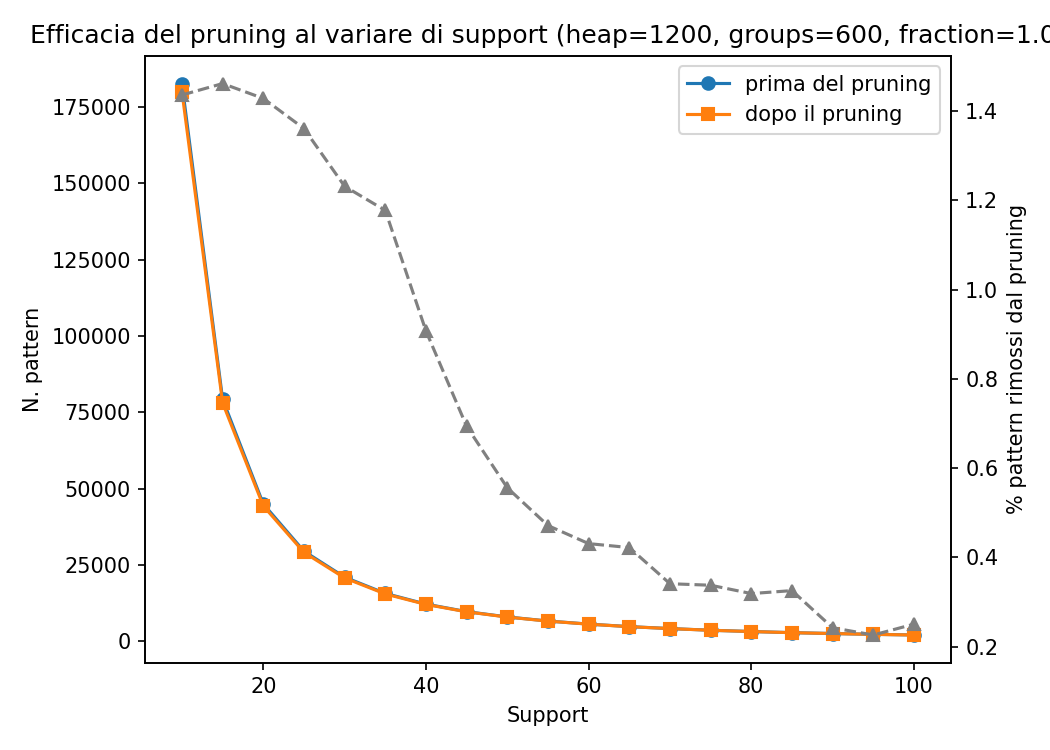
\includegraphics[width=\columnwidth]{3_pruning_vs_support.png}
    \caption{Pattern count before (blue) and after (orange) Transitive
        Modulo Pruning as a function of minimum support, with the removal
        percentage on the right axis (dashed). The pruning rate remains
        below $1.5\%$ across all configurations.}
    \label{fig:pruning_support}
\end{figure}

\subsection{Scalability of the Pruning Phase}

Figure~\ref{fig:pruning_scalability} shows the absolute execution time
of the pruning phase as a function of input pattern count, on a log-log
scale. Below approximately $10{,}000$ patterns, pruning time remains
sub-second with moderate variance attributable to Spark task scheduling
jitter. Beyond this threshold, execution time increases more steeply
and variance grows substantially, reaching 2--3 seconds at
$\sim\!150{,}000$ patterns.

The observed growth is consistent with the $\mathcal{O}(|\alpha|^2)$
pairwise divisibility check performed within each canonical shape group
by \texttt{reduce\_alpha\_edges}: as the number of distinct scaling
factors per group increases, the local quadratic cost dominates.
However, because \texttt{groupByKey} ensures each group is processed
independently on a single worker, this cost does not propagate globally
— the pruning phase remains parallelisable across shape groups and its
wall-clock time is bounded by the largest individual group rather than
the total pattern count.

\begin{figure}[H]
    \centering
    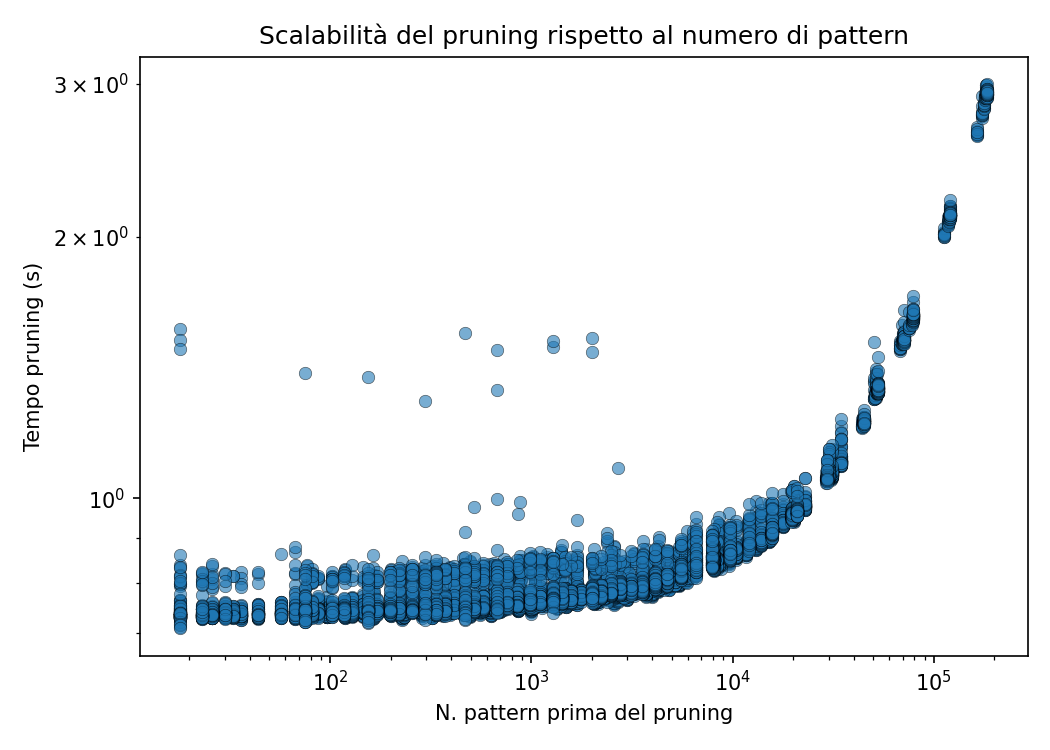
\includegraphics[width=\columnwidth]{6_scalabilita_pruning.png}
    \caption{Pruning phase execution time as a function of input pattern
        count (log-log scale). Time remains sub-second below
        $\sim\!10{,}000$ patterns and grows toward 2--3 seconds at
        $\sim\!150{,}000$, consistent with the local quadratic cost of
        pairwise divisibility checks within each canonical shape group.}
    \label{fig:pruning_scalability}
\end{figure}

% ============================================================
\section{Limitations and Conclusion}
\label{sec:limitations}
% ============================================================

\subsection{Limitations and Future Work}

While the proposed pipeline successfully extracts structural proportions from
massive datasets, several constraints remain that offer opportunities for
future research:

\begin{itemize}
    \item \textbf{Sensitivity to Quantity Noise:} The reliance on the GCD for
          extracting the Scaling Factor ($\alpha$) makes the model highly sensitive to
          noise in purchase quantities. A minor deviation in a single transaction
          (e.g., a user purchasing $11$ units instead of $10$) can prevent the discovery
          of a $1{:}2$ ratio, as the integer factorisation logic is strict. Future
          iterations could incorporate a fuzzy GCD or clustering-based approach to
          handle near-proportionality.

    \item \textbf{Strict Proportionality Constraints:} The current model
          assumes that consumer behaviour scales linearly ($P = \alpha \cdot S$). It does
          not account for non-linear trends, such as bulk-buy behaviours where product
          ratios might shift as total volume increases.

    \item \textbf{Absence of Temporal Analysis:} The pipeline processes the
          dataset as a static snapshot. It does not currently capture seasonal variations
          or time-based shifts in purchase proportions, which are critical for dynamic
          retail environments.

    \item \textbf{Local Execution Environment:} All experiments were conducted
          on a single machine in Spark's \texttt{local[*]} mode. While this validates
          algorithmic correctness and relative scaling behaviour, it does not replicate
          the inter-node communication patterns and network overhead of a true
          distributed cluster. Deployment on a cloud infrastructure such as Azure
          HDInsight or Amazon EMR would be required to validate the near-linear speedup
          claim at industrial scale.
\end{itemize}

\subsection{Conclusion}

This work has successfully extended the traditional Frequent Itemset Mining
(FIM) paradigm by introducing a distributed framework for proportional
quantitative analysis. By leveraging the Parallel FP-Growth (PFP) engine, we
have demonstrated that it is possible to move beyond simple binary associations
to uncover the underlying structural ratios of consumer behaviour without
sacrificing computational scalability.

Our implementation introduced three key technical contributions:

\begin{itemize}
    \item \textbf{Bijective Token Indexing:} A transformation layer that allows
          the PFP distributed engine to process quantitative tuples while maintaining
          compatibility with standard prefix-tree structures.

    \item \textbf{Structural Decomposition:} A mathematical approach, anchored
          in the Prefix Path Property of FP-trees, that utilises integer factorisation to
          detach a pattern's irreducible Canonical Shape from its scalar magnitude.

    \item \textbf{Topological Synthesis:} A post-processing phase that applies
          Transitive Modulo Pruning to eliminate redundant informational pathways,
          transforming a flat list of patterns into an optimised Directed Acyclic Graph
          (DAG).
\end{itemize}

The performance analysis, conducted on the Dunnhumby \textit{The Complete
Journey} dataset, confirms that the mining phase achieves near-linear scaling
with respect to dataset size, while the Proportional Graph Construction phase
adds at most $6\%$ overhead to total execution time. Pipeline correctness was
verified end-to-end through a synthetic worked example exercising both the
multi-parent convergence and linear scaling topologies. By providing an Atlas
of Proportionality rather than a simple list of popular items, this system
empowers businesses with deeper insights for automated bundle recommendations
and targeted inventory management, effectively bridging the gap between big
data mining and actionable business intelligence.



\end{document}
